% urban-short-report.tex
% v0.1 Sept. 2021

\documentclass{urban-formatting}

\begin{document}
%%%%%%%%%%%%%%%%%%%%%%%%%%%%%%%%%%%% Title %%%%%%%%%%%%%%%%%%%%%%%%%%%%%%%%%%%%%%

\begin{titlepage}
    % Add logo
    \begin{textblock*}{8.5in}(0in, 0.15in)
        \begin{tcolorbox}[valign = center]
            \begin{center}
                \policycenter{[Policy Center, Initiative, or Taxonomy Terms Here]}
            \end{center}
        \end{tcolorbox}
    \end{textblock*}

    % Adding the cover image - code forces the image to be width of full paper (ignoring margins)
    \vspace*{-1.5cm}
    \noindent
    \makebox[\textwidth]{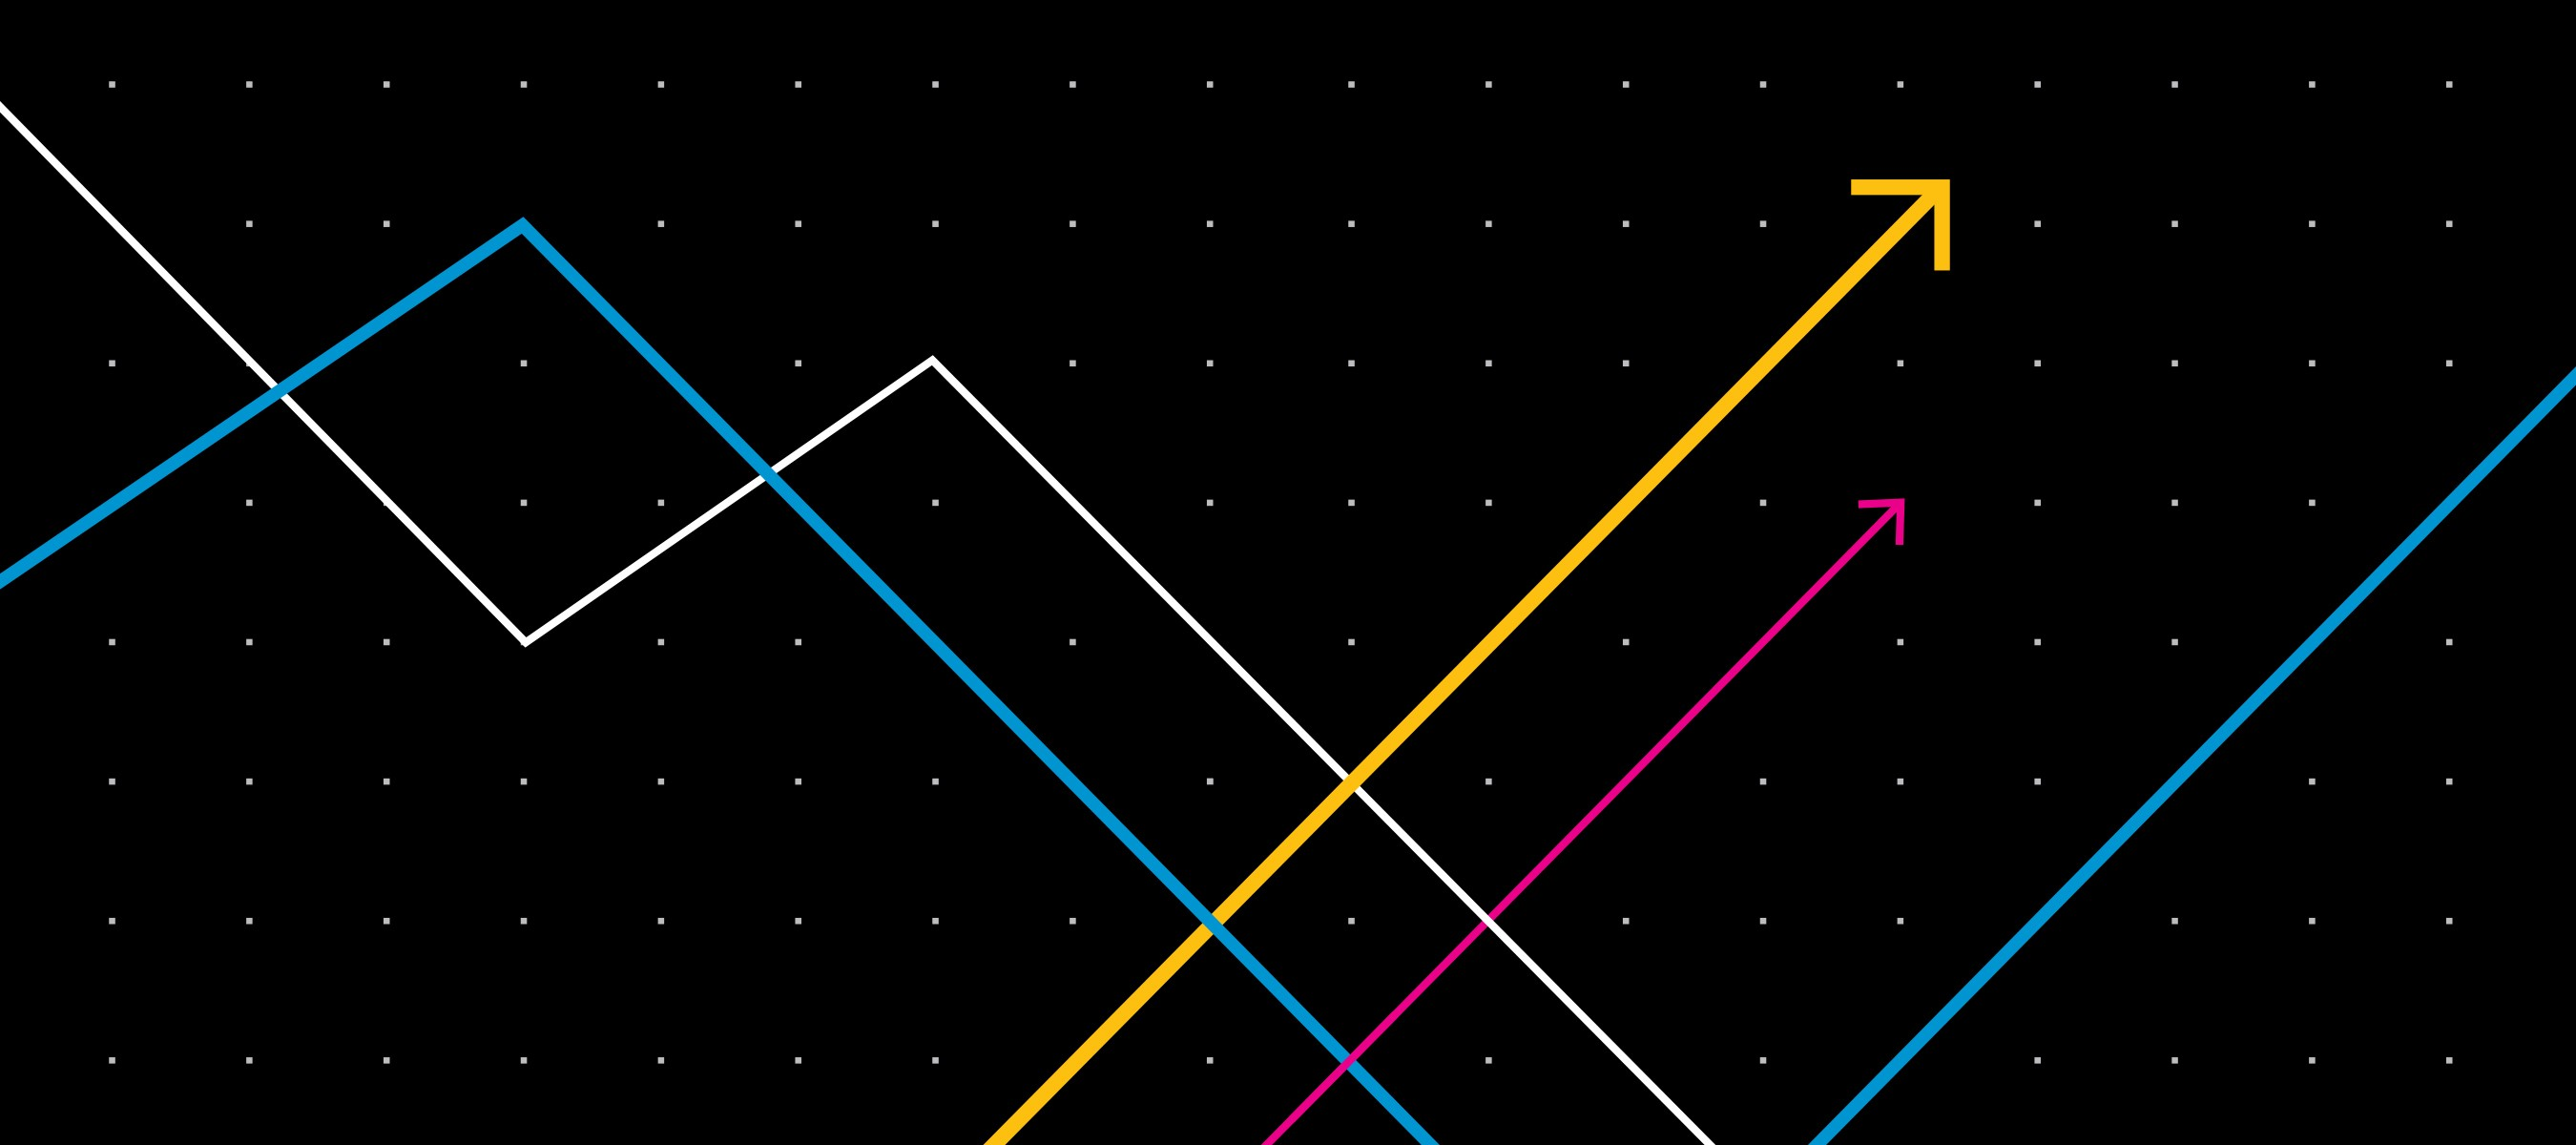
\includegraphics{images/cover.jpg}}
    
    \vspace{0.3in}
    \noindent\textcolor{urban-cyan}{\MakeUppercase{\textbf{Research Report}}}
    
    \titlereport{Title Here in Title Case}
    
    \reportsubtitle{Subtitle Here in Title Case}
    
    % Multiple column author names - change the "4" to the number of desired columns
    \begin{multicols}{4}
        \authorfont{Author 1 Name}\\
        \affiliationfont{Author's Affiliation}
        
        \authorfont{Author 2 Name}\\
        \affiliationfont{Author's Affiliation}
        
        \authorfont{Author 3 Name}\\
        \affiliationfont{Author's Affiliation}
        
        \authorfont{Author 4 Name}\\
        \affiliationfont{Author's Affiliation}
    \end{multicols}
    
    \vspace{-0.5cm}
    \authorfont{with Author Name and Author Name}
    
    \datefont{Month and Year}
    \vfill
    \vfill
    \vfill
    
    % Add logo
    \begin{textblock*}{5in}[1, 1](6in, 10.5in)
        \noindent
\includegraphics[width=5in]{images/cover-footer.jpg}
    \end{textblock*}
\end{titlepage}

%%%%%%%%%%%%%%%%%%%%%%%%%%%%%%%%%%%% About Urban %%%%%%%%%%%%%%%%%%%%%%%%%%%%%%%%%%%%%%
\newpage
\thispagestyle{empty} % Removed Page Number
\begin{figure}
    
\includegraphics[width=1.5in]{images/logo.png}
\end{figure}
\vspace*{-0.5in}
\about{About the Urban Institute}\\
\boilerplate{The nonprofit Urban Institute is a leading research organization dedicated to developing evidence-based insights that improve people’s lives and strengthen communities. For 50 years, Urban has been the trusted source for rigorous analysis of complex social and economic issues; strategic advice to policymakers, philanthropists, and practitioners; and new, promising ideas that expand opportunities for all. Our work inspires effective decisions that advance fairness and enhance the well-being of people and places.}

\vspace*{\fill}
\noindent Copyright ©\tbf{Month Year}. Urban Institute. Permission is granted for reproduction of this file, with attribution to the Urban Institute. Cover image by \tbf{Tim Meko}.

%%%%%%%%%%%%%%%%%%%%%%%%%%%%%%%%%%%% Contents %%%%%%%%%%%%%%%%%%%%%%%%%%%%%%%%%%%%%%
\newpage
\tableofcontents

%%%%%%%%%%%%%%%%%%%%%%%%%%%%%%%%%%%% Acknowledgments %%%%%%%%%%%%%%%%%%%%%%%%%%%%%%%%%%%%%%
\newpage
\part*{Acknowledgments}

This report was funded by \tbf{[insert your funder name(s) here].} We are grateful to them and to all our funders, who make it possible for Urban to advance its mission. 

The views expressed are those of the \tbf{author/authors} and should not be attributed to the Urban Institute, its trustees, or its funders. Funders do not determine research findings or the insights and recommendations of Urban experts. Further information on the Urban Institute’s funding principles is available at urban.org/fundingprinciples.

\tbf{[Add any other thanks and contract details here. It may be appropriate to also acknowledge your funder’s funder(s). When in doubt, please check with your center director and Contracts.]}

%%%%%%%%%%%%%%%%%%%%%%%%%%%%%%%%%%%% Executive %%%%%%%%%%%%%%%%%%%%%%%%%%%%%%%%%%%%%%
\newpage
\part*{Executive Summary}

\intropara{Body Text style or Chapter Intro Para style here (text shown is in Chapter Intro Para). If you do not have an executive summary, remove this section.}

\section*{First-Level Heading in Title Case (Heading 2 style)}

Body Text style for first paragraph under a heading.

Body Text First Indent style for all subsequent paragraphs. \tbf{To add an endnote, use the Insert Endnote function. Endnotes will automatically appear in the Notes section after the appendixes.}

\subsection*{Second-Level Heading in Title Case (Heading 3 style)}

Body Text style for first paragraph under a heading.

Body Text First Indent style for all subsequent paragraphs.


\subsubsection*{THIRD-LEVEL HEADING; ALL CAPS IS BUILT INTO STYLE (HEADING 4 STYLE)}

Body Text style for first paragraph under a heading.

Body Text First Indent style for all subsequent paragraphs.


%%%%%%%%%%%%%%%%%%%%%%%%%%%%%%%%%%%% About Author %%%%%%%%%%%%%%%%%%%%%%%%%%%%%%%%%%%%%%
\newpage
\part*{About the Authors}
\textbf{Author Name in Bold} but the rest of the text lightface. Use Author Bios--First style for the introductory paragraph of each bio. You can paste your bio from your author page on the Urban website (and condense it if needed) here. 

If your bio is more than one paragraph long, use Author Bios--Additional for any subsequent paragraphs. This style suppresses spacing between paragraphs.

Author bios no longer include photos.


%%%%%%%%%%%%%%%%%%%%%%%%%%%%%%%%%%%% Back Cover %%%%%%%%%%%%%%%%%%%%%%%%%%%%%%%%%%%%%%
\newpage
\thispagestyle{empty}

\begin{textblock*}{8.5in}[1, 1](8.5in, 11in)
    \noindent
\includegraphics[width=\paperwidth,height=\paperheight]{images/back.pdf}
\end{textblock*}

\end{document}
